\chapter{系统实现}\label{chap:implementation}

\section{前端实现}

微信小程序前端作为校内综合交通平台的统一用户入口，采用微信原生小程序框架实现，项目主体位于TJ-Transport目录下。前端工程以页面、组件、服务接口和工具函数为主要组织方式，通过app.json完成页面注册、底部导航栏配置、渲染模式设置和权限声明。系统将论坛、交通、拼车、消息和个人中心设置为五个一级页面，并通过tabBar固定在底部导航区域，使用户能够在不同业务模块之间进行快速切换。页面层主要负责界面状态维护和用户交互响应，服务层负责接口调用和数据结构转换，组件层负责可复用界面单元的封装。该实现方式避免了页面脚本直接处理后端原始数据，使前端页面能够面向统一的视图模型进行渲染，从而降低不同微服务返回字段差异对页面逻辑的影响。为展示小程序前端各主要功能入口及页面组织方式，系统核心页面实现效果如\figref{fig:mini-program-pages}所示。

\begin{figure}[!htbp]
  \centering
  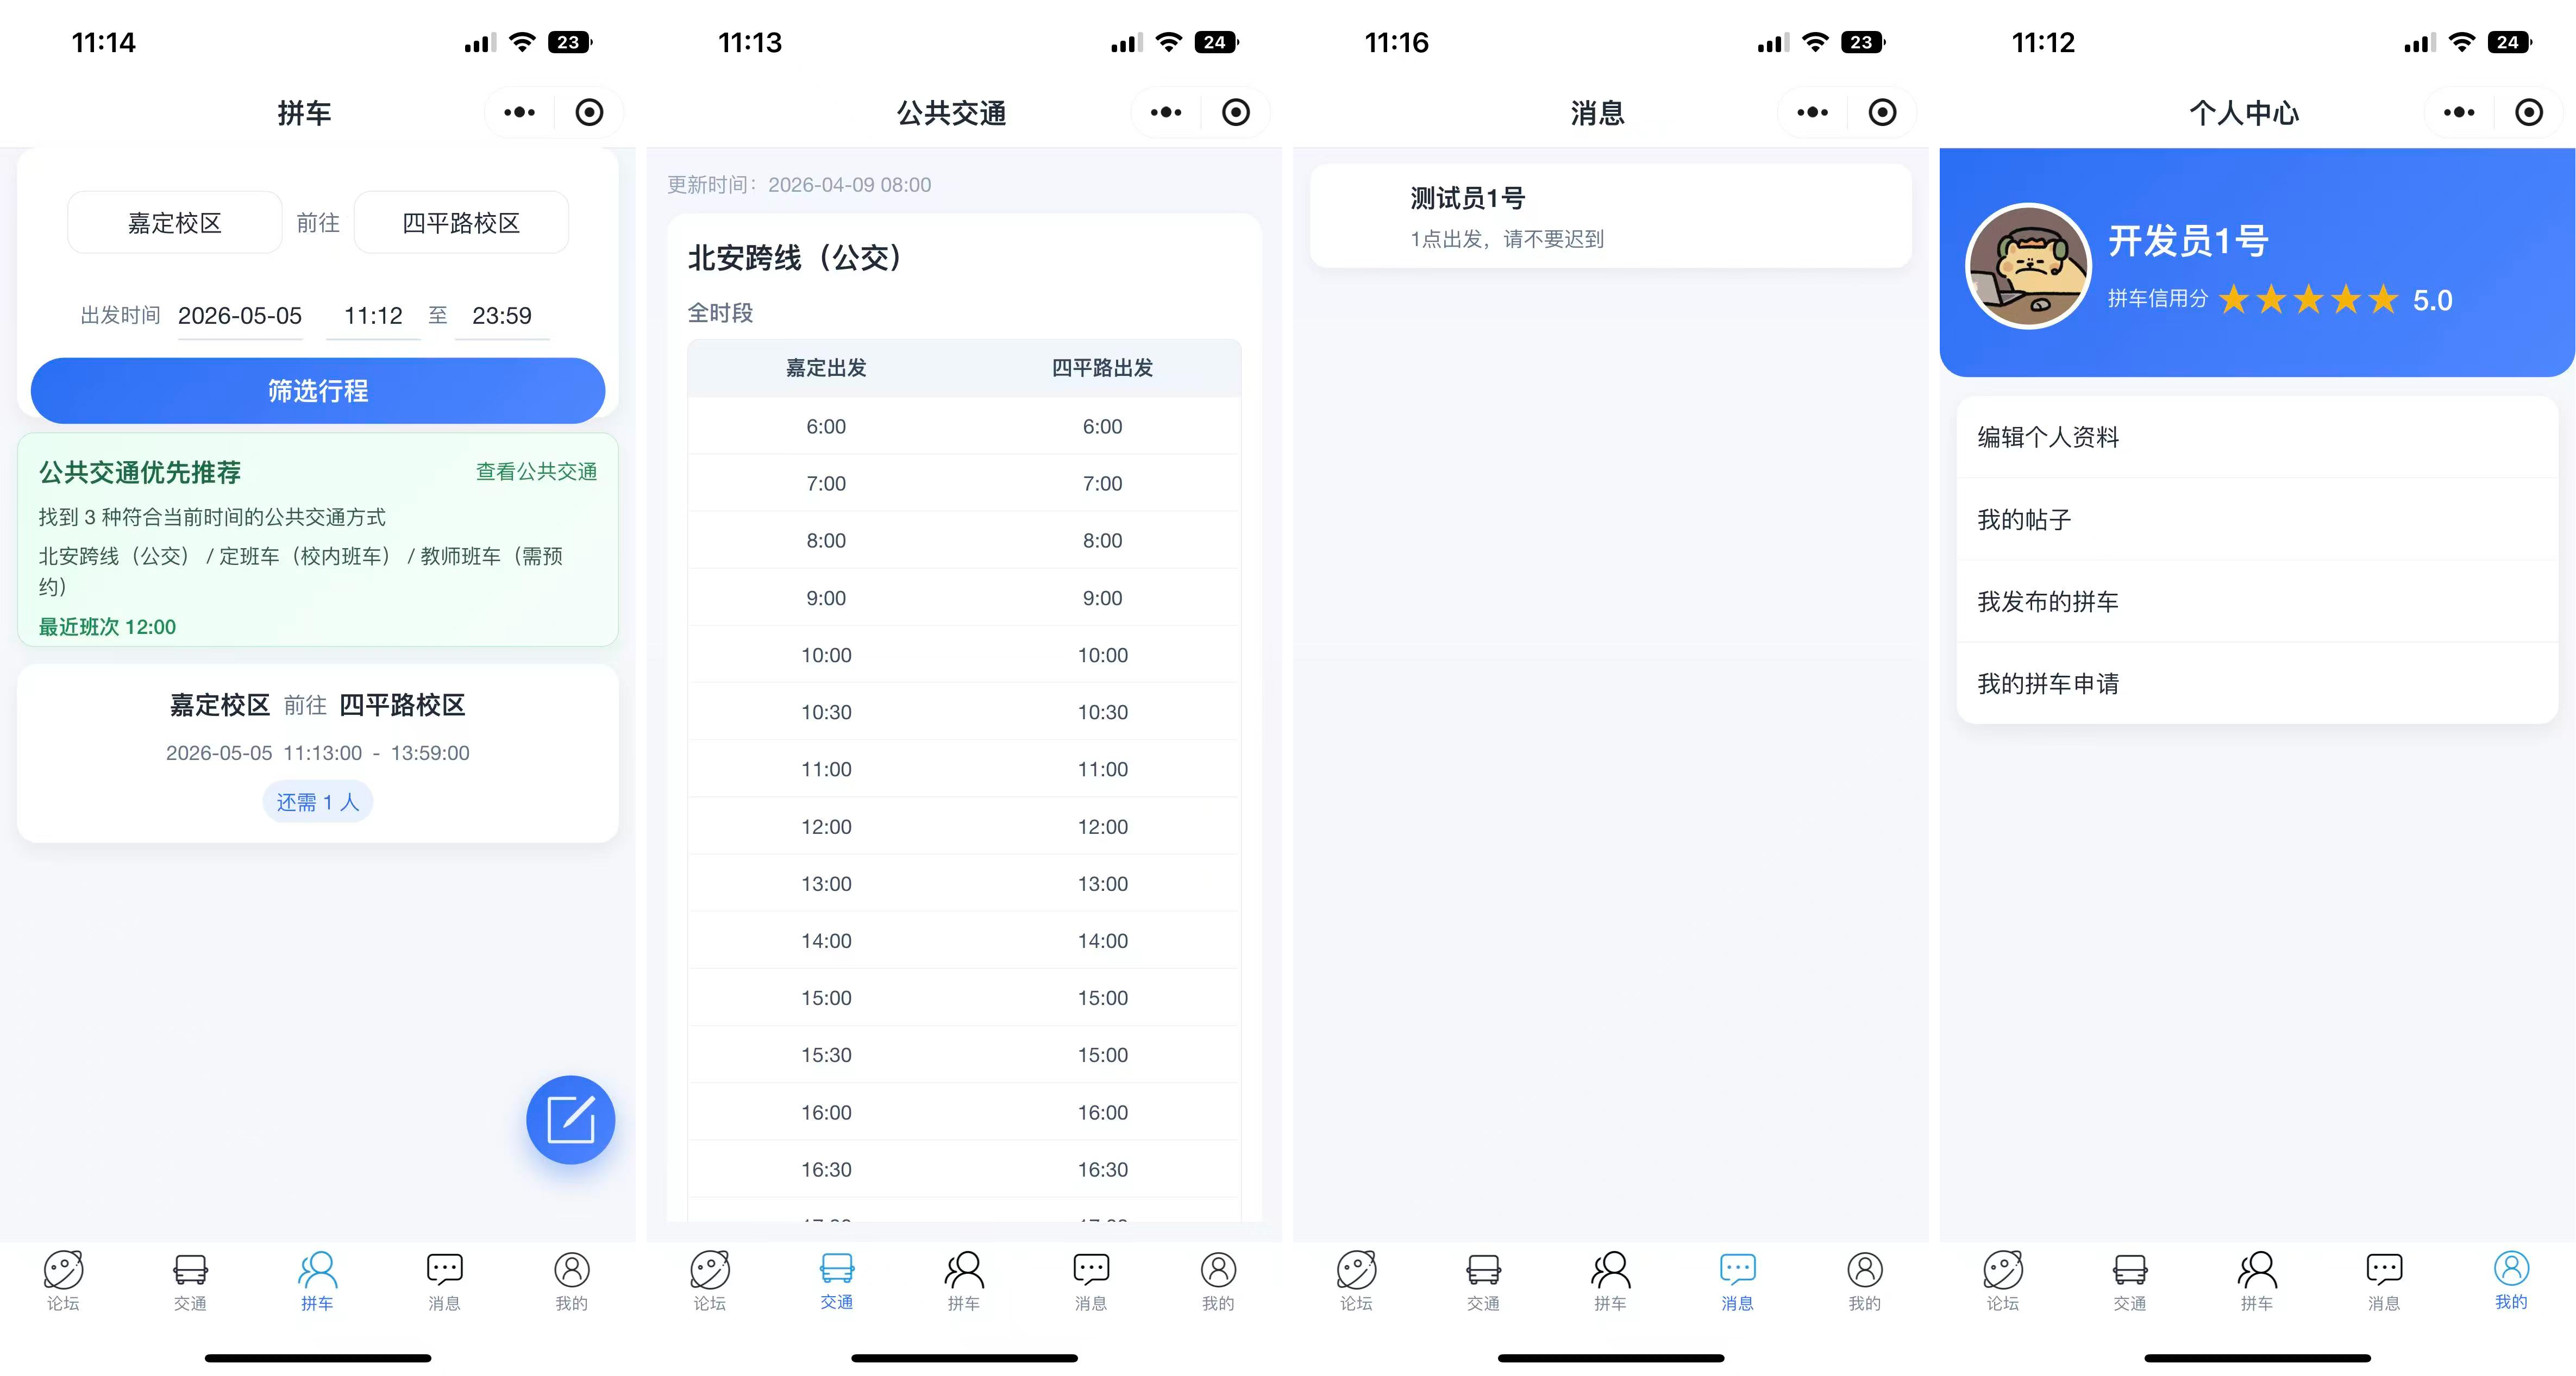
\includegraphics[width=0.9\textwidth]{figures/fig-5-1-mini-program-pages.png}
  \caption{小程序主要页面实现效果图}
  \label{fig:mini-program-pages}
\end{figure}

在数据请求实现方面，前端并未在各页面中直接调用wx.request，而是通过utils/request.js进行统一封装。该模块依据请求路径前缀对不同业务进行分发，将请求转发至对应的后端服务接口，同时统一设置请求头并对响应结果进行规范化处理。当请求成功且业务code为0时返回有效数据，否则构造统一的异常对象供调用方处理。通过这一方式，页面层无需重复编写状态判断与错误处理逻辑，从而将关注点集中于业务数据本身，提高了代码的一致性与可维护性。

在接口管理与数据适配方面，系统通过api/endpoints.js对各模块接口地址进行集中定义，各业务service文件在调用时统一引用该配置，避免在页面中直接书写具体路径。在此基础上，服务层对后端返回数据进行结构转换，将原始字段映射为前端统一使用的视图字段。例如拼车模块在处理订单数据时，会将后端字段转换为页面所需的数据结构，从而保证页面模板的数据绑定格式保持稳定。当后端接口字段发生变化时，仅需在服务层进行调整即可完成适配，降低了前端页面的修改成本。

页面状态管理依赖于微信小程序Page对象中的data与setData机制实现。页面通过data维护输入内容、列表数据及各类状态信息，并通过事件回调对局部状态进行更新。在实际实现中，列表页面通常结合分页与下拉刷新机制进行数据管理，通过控制加载状态避免重复请求，并在数据更新后同步刷新视图。同时，搜索等交互操作通过组件触发事件，将用户输入传递至页面并重新发起数据请求，从而实现条件变化与数据展示之间的动态联动。组件复用是该前端工程实现中的重要特征。系统将页面中高频出现的界面元素进行抽象封装，通过组件统一管理展示逻辑与交互行为。组件通过properties接收页面传入的数据，并利用observers将外部数据同步至内部状态，同时通过triggerEvent向父页面传递用户操作事件。在具体实现中，列表项展示、搜索输入以及聊天气泡等均通过组件完成，页面仅需提供必要的数据对象即可实现渲染与交互。这种方式将通用界面逻辑从页面中剥离，使页面脚本能够更加专注于业务流程与数据请求，同时也提升了模板结构的清晰度与代码复用程度。

在表单与媒体处理方面，前端主要依赖微信小程序提供的原生能力实现。论坛发帖功能通过接口选择本地图片，并在必要时进行压缩处理后加入待上传列表，随后由服务层逐步完成文件上传并获取远程资源地址，再提交帖子数据。在数据提交之前，页面会对标题、内容及相关字段进行校验，从源头避免无效数据进入后端。同时，前端支持图片预览功能，使用户在提交前能够直观确认内容。在拼车相关操作中，系统通过订阅消息授权机制，将关键业务操作与通知能力进行结合。整体而言，表单输入、媒体处理与数据提交均通过页面事件与服务层方法协同完成，使前端在承担界面展示的同时，也具备必要的数据约束与流程控制能力。

总体来看，微信小程序前端采用页面、服务与组件分层的实现结构。页面层负责状态管理与交互控制，通过生命周期函数完成数据初始化与更新，并利用setData实现视图驱动；服务层统一封装接口调用与数据转换，屏蔽后端差异；组件层则负责界面复用与局部交互封装。通过这一结构，不同功能模块在同一工程中保持一致的实现方式，使系统在扩展与维护过程中具备较好的结构稳定性与边界清晰性。

\section{后端实现}

\subsection{后端系统架构与服务设计}

本系统后端采用按业务功能划分的多服务架构设计，不同业务模块以独立的Spring Boot工程形式进行组织，涵盖用户管理、拼车服务、社区交流、即时通信和公共交通等功能。各服务通过HTTP接口与前端及其他服务进行交互，实现功能模块在工程层面的相对独立，避免了单一系统中不同业务逻辑的过度耦合，同时为后续维护与扩展提供了清晰边界。

在代码组织方面，各服务内部采用典型的分层结构，包括控制层、业务层、数据访问层、持久化模型以及数据传输对象。控制层负责接收请求并完成参数解析，业务层实现核心业务逻辑，数据访问层负责与数据库交互，模型层与持久化对象对应，数据传输对象用于封装响应数据。通过这一分层方式，接口接入、业务计算和数据存储职责被明确划分，使系统在功能扩展和维护中具有较高的可管理性。

后端服务对外提供REST风格接口，前端通过HTTP请求访问各模块功能。接口参数根据具体业务场景通过请求体或查询参数传入，控制层完成基础类型转换后，将业务处理交由业务层执行。为保证前后端交互的一致性，系统定义了统一的响应对象，接口正常返回时包含状态码、提示信息和业务数据，异常情况下返回非成功状态及错误信息。统一响应结构降低了前端适配不同服务响应的复杂度，并保证了接口错误处理的一致性。系统还通过集中式异常处理机制，将业务层抛出的常见运行时异常转化为标准化响应，避免将内部堆栈信息暴露给前端，从而实现业务校验逻辑集中化，接口层保持简洁。

服务间调用方面，系统通过封装客户端类实现微服务之间的数据交互。例如，拼车服务在需要获取用户信息时通过调用用户服务接口补全订单发布者及申请者资料，论坛服务同样通过用户服务获取作者信息；在调用外部机器学习模型服务进行拼车匹配排序时，则通过客户端向模型服务发送特征向量并接收预测结果。通过客户端封装，业务服务无需直接处理具体HTTP请求，实现调用逻辑与业务逻辑的解耦，并能够在调用异常时进行降级处理。

在一致性控制方面，单服务内部通过事务机制保证关键操作的原子性，例如拼车申请审批、订单完成及反馈提交等涉及多条数据更新的操作。在跨服务数据更新场景中，例如提交反馈后更新用户信用统计，系统采用“先保存业务记录，再调用用户服务更新统计”的方式实现逻辑一致性。虽然该方式不是严格的分布式事务，但在本系统规模和业务场景下能够满足实际需求，并降低系统实现的复杂度。

\subsection{用户服务实现}

用户服务主要负责小程序用户身份维护、基础资料管理以及拼车相关信用信息的统计与更新。在登录流程中，前端通过调用微信登录接口获取临时凭证后提交至后端，用户服务根据唯一标识判断用户是否已存在，并据此执行更新或创建操作，从而完成用户身份的初始化与维护。用户信息统一存储于关系型数据库中，包含基本资料字段及与拼车行为相关的统计信息。

在功能实现上，用户服务不仅提供资料查询与更新能力，还承担用户信用指标的维护职责。当拼车服务产生评价数据后，会调用用户服务接口传递评分、迟到情况及行程完成情况等信息。用户服务基于历史统计结果进行累计更新，动态计算用户信用值及相关比例指标，使用户信用能够随实际行为持续变化。这些统计结果同时作为拼车匹配过程中的重要参考特征。

在数据访问层，系统通过数据访问框架对数据库进行操作，实现对用户信息的查询与更新。常用的数据访问方法通过接口形式定义，从而减少基础数据操作代码的重复编写，使实现重点集中在登录逻辑、资料维护及信用统计等核心业务处理上。

\subsection{拼车服务实现}

拼车服务是系统中业务约束较为复杂的核心模块，主要围绕拼车订单、申请处理及行程反馈等功能展开。在订单创建过程中，系统对用户身份、出发与到达地点、出行时间区间以及座位数量等信息进行校验，确保数据满足基本业务规则后，将订单写入数据库并记录相关时间信息。

在申请处理方面，系统通过一系列约束条件保证业务逻辑的一致性。用户提交申请时，需满足订单仍处于可加入状态且存在剩余座位等条件，同时避免同一用户对同一订单重复提交申请。在订单发布者对申请进行处理时，系统根据审批结果同步更新申请状态及订单剩余座位数量，并通过事务机制保证相关数据在更新过程中的一致性。

在行程完成后，系统支持参与用户之间的评价机制。拼车服务根据订单参与关系确定评价对象范围，并在提交评价时对数据合法性进行校验，防止重复评价或非法操作。评价数据保存后，服务通过接口调用将相关信息传递至用户服务，用于更新用户信用统计。通过这种方式，实现了拼车行为与用户信用之间的关联。

\subsection{论坛服务实现}

论坛服务用于支持帖子发布、列表查询、详情查看以及评论与点赞等功能。该模块采用文档型数据库进行数据存储，将帖子、评论与点赞记录分别组织为独立集合。帖子数据中包含正文内容、标签信息及附件列表，能够较好地适应内容结构灵活变化的特点，从而满足校园交流场景中多样化的数据需求。

在帖子创建过程中，服务接收前端提交的标题、内容、标签及图片地址等信息，对图片数据进行封装处理后与其他字段一并写入数据库，同时初始化相关统计字段。帖子列表查询支持关键字搜索与标签筛选，并结合分页与时间排序机制返回结果。为满足前端展示需求，服务在返回数据时通过调用用户服务获取发帖人相关信息，并将其整合至响应结构中。

在交互功能实现方面，系统通过记录行为数据与维护计数字段相结合的方式处理点赞与评论操作。当用户执行点赞或取消点赞操作时，系统同步更新对应记录与统计值；评论的新增与删除亦采用类似机制。通过在帖子对象中维护计数信息，避免在列表查询时对评论或点赞数据进行实时统计，从而提高数据读取效率。

\subsection{聊天服务实现}

聊天服务主要实现用户之间的会话管理与消息交互功能，采用文档型数据库存储会话与消息数据。会话数据用于描述参与用户及相关状态信息，消息数据则记录具体的通信内容及其状态属性。通过这种结构划分，可以在保持数据灵活性的同时支持多用户状态的独立维护。

在会话创建过程中，系统根据参与用户关系判断是否已存在对应会话，若存在则直接复用，否则创建新的会话记录，并初始化参与者信息。消息发送时，服务首先对发送者身份进行校验，随后生成消息数据并写入数据库，同时更新会话的时间信息，以便后续按最近活动进行排序。

在消息读取与状态管理方面，系统根据会话标识获取对应消息列表，并按照时间顺序返回。对于用户已删除或已读的消息状态，通过在消息数据中维护对应标记进行控制。用户进入会话后，系统对相关消息进行已读状态更新，从而保证会话列表与消息状态的一致性。该实现方式在不引入复杂通信机制的情况下，实现了基本的即时通信功能，并能够支持用户对消息状态的个性化管理。

\subsection{文件服务实现}

文件服务主要用于支持论坛图片上传及后续文件访问。前端在选择文件后，通过接口将文件提交至服务端，服务接收文件并记录相关元数据。系统中，文件记录对象包含上传用户、文件名、类型、大小、上传时间、是否永久保存及过期时间等信息。实际文件的存储逻辑被封装在专门的存储服务中，并提供本地存储实现。通过将文件记录与存储逻辑分离，系统在后续扩展到对象存储或云存储时能够保持接口层的稳定性与一致性，从而简化功能扩展和维护。

\subsection{交通服务实现}

交通服务主要负责公共交通和校车时刻表数据的查询与管理。该服务采用文档型数据库存储时刻表信息，文档包含更新时间、线路、区段及具体时间行等多层嵌套结构。通过数据库直接保存嵌套数据，系统能够完整反映线路与区段之间的层级关系，并支持前端按照线路与区段展示完整的出行时间信息。服务在读取数据后会将文档转换为前端所需的响应结构，使前端能够直接进行可视化展示，从而满足校园公共交通及班车信息查询需求。

\section{拼车匹配算法实现}

\subsection{二层匹配机制总体设计}

拼车匹配算法是拼车服务中连接用户出行需求与已有拼车订单的核心部分。系统在实现时没有直接将所有订单交由机器学习模型处理，而是采用“规则筛选+随机森林排序”的二层匹配机制。该机制的主要考虑在于，校园拼车场景中的起点、终点、日期、时间和座位余量具有明确的业务约束，如果不满足这些基础条件，即使模型预测分数较高，也不应作为有效候选结果展示。因此，算法先通过确定性规则缩小候选订单范围，再对候选结果进行综合评分与模型重排，从而兼顾业务可解释性和排序效果。为便于说明拼车匹配算法在系统运行过程中的执行路径，本文绘制其在线处理流程，如\figref{fig:matching-flow}所示。

\begin{figure}[!htbp]
  \centering
  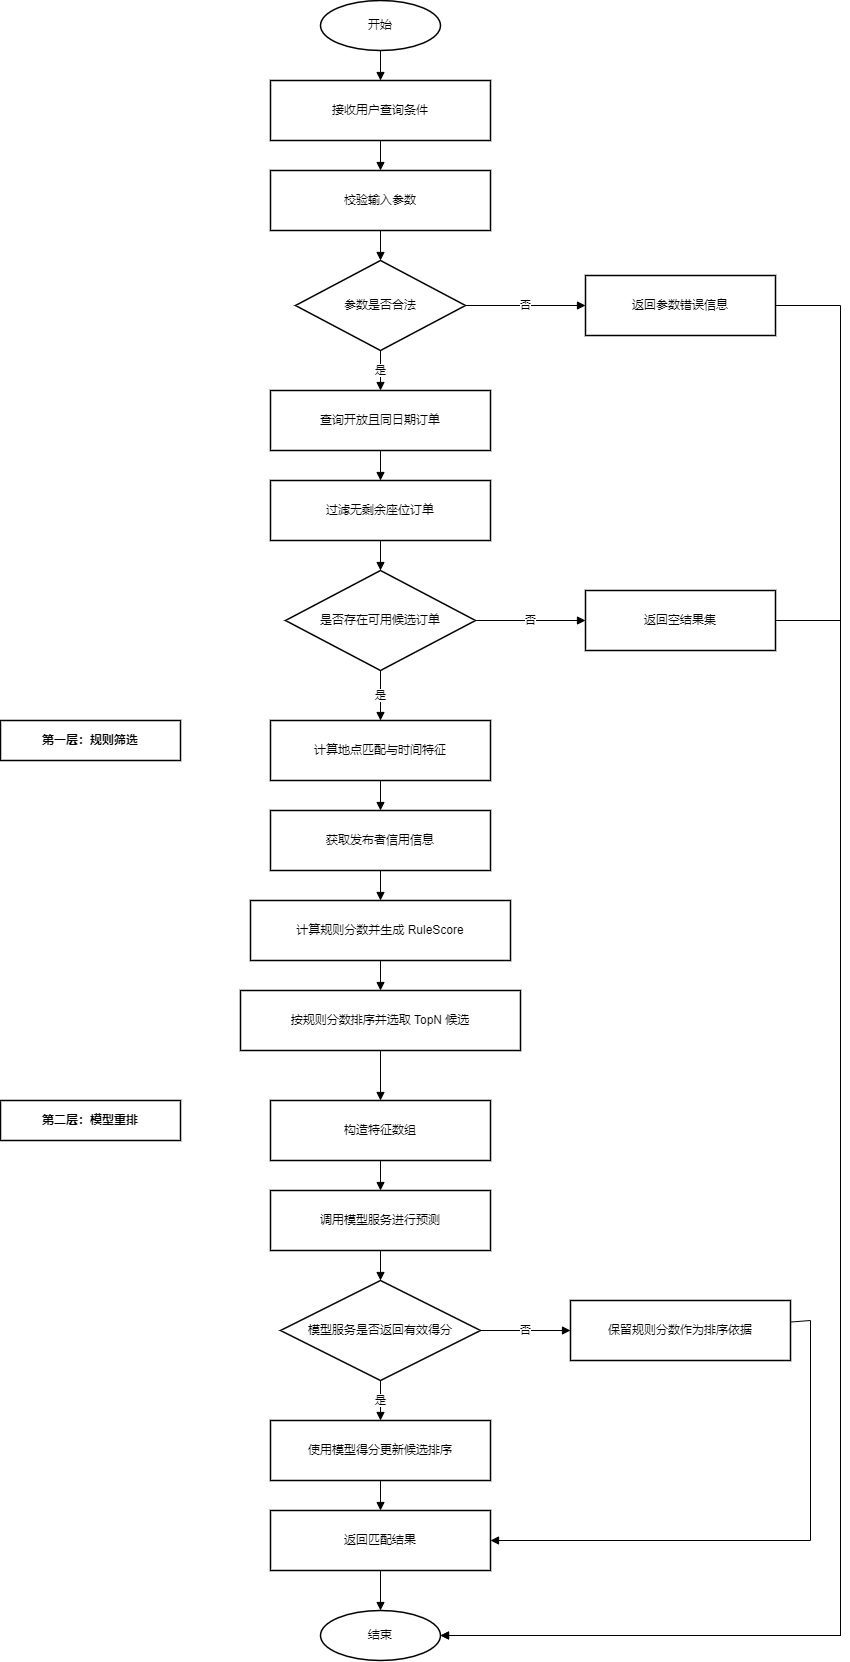
\includegraphics[width=0.56\textwidth]{figures/fig-5-2-matching-flow.png}
  \caption{拼车匹配算法在线执行流程图}
  \label{fig:matching-flow}
\end{figure}

\subsection{规则筛选层实现}

规则筛选层的主要作用在于保证匹配结果在业务层面的可行性。当用户提交拼车查询请求后，后端首先对输入参数进行合法性校验，包括地点是否属于系统预设范围、时间区间是否有效以及起止时间关系是否合理。通过对地点集合进行限定，可以避免非规范输入对匹配结果造成干扰，从而提高整体数据的一致性。

在候选订单获取阶段，系统仅从数据库中筛选状态为开放且出行日期匹配的订单，并进一步过滤仍有剩余座位的记录，以保证进入匹配流程的订单均具备可加入条件。在此基础上，系统对候选订单的空间与时间特征进行计算。空间匹配采用离散方式，根据起点与终点的一致性或近似程度进行量化，并仅保留同时满足起点与终点匹配要求的订单。时间匹配则通过比较两个时间区间的重叠情况进行衡量，重叠程度越高表示时间匹配程度越好；当时间区间不存在交集时，订单将被直接排除。同时，系统还通过时间区间中心点差值反映出行时间的偏移程度，并构造相应标记用于描述基本时间兼容性。

在完成筛选与特征计算后，规则层进一步对候选订单进行初步评分。评分过程综合考虑空间匹配、时间匹配以及发布者的历史信用情况等因素，通过加权方式生成初始匹配分数，并对结果进行归一化处理。该分数既用于对候选订单进行基础排序，也作为后续模型排序或模型不可用时的参考依据，从而在整个匹配流程中起到承上启下的作用。

\subsection{随机森林模型设计}

规则筛选虽然能够保证匹配结果的基本合理性，但单纯依赖人工权重难以充分表达不同特征之间的非线性关系。例如，当地点完全匹配但时间偏移较大时，订单是否应排在前列，需要同时考虑时间重叠比例、中心差和用户信用；当时间完全匹配但发布者迟到率较高时，也需要对排序结果进行适当调整。为提高排序的灵活性，系统在规则筛选后引入随机森林回归模型，对候选订单进行二次评分。

随机森林是一种基于集成学习思想的模型，其核心思想是构建多棵决策树，并通过多棵树的预测结果综合得到最终输出。对于回归任务，随机森林通常取各决策树预测值的平均作为最终结果。与单棵决策树相比，随机森林通过样本扰动和特征扰动降低模型方差，能够提高泛化能力。同时，随机森林不要求输入特征满足线性关系，也不依赖特征归一化，对校园拼车中同时包含匹配度、时间差、信用分和迟到率等不同类型特征的场景较为适用。

本系统将随机森林模型设计为回归模型，输出值表示候选订单与用户需求之间的匹配得分。模型输入包含8个特征，依次为startMatch、endMatch、timeOverlap、timeCenterDiff、isTimeCompatible、userCredit、successRate和lateRate。其中，startMatch和endMatch表示起点与终点匹配程度；timeOverlap表示时间重叠比例；timeCenterDiff表示两个时间区间中心点之间的差值；isTimeCompatible表示是否存在时间交集；userCredit表示发布者信用分；successRate表示发布者历史拼车完成率；lateRate表示发布者历史迟到率。上述特征覆盖了空间、时间和用户可靠性三个维度，能够较全面地描述候选订单质量。

\subsection{模型训练过程}

由于系统在开发阶段缺少大规模真实历史拼车行为数据，模型训练采用模拟数据生成方式构造训练集。数据生成脚本按照拼车业务特征随机生成样本，其中startMatch、endMatch和timeOverlap在0到1之间取值，timeCenterDiff取0到120分钟之间的整数，isTimeCompatible根据timeOverlap是否达到一定条件确定，userCredit在0.5到1之间取值，successRate在0.3到1之间取值，lateRate在0到0.5之间取值。目标匹配分数由加权评分函数生成，并加入小幅随机扰动，以模拟真实用户选择行为中的不确定性。

训练阶段采用RandomForestRegressor作为模型主体。系统读取训练数据后，将前8列作为特征矩阵，将最后一列匹配分数作为目标值。训练集与测试集按照8:2的比例划分，random\_state设置为42，以保证实验结果可复现。模型参数中，n\_estimators设置为150，表示随机森林包含150棵决策树；max\_depth设置为12，用于限制单棵树深度，避免模型过度拟合模拟样本。训练完成后，系统使用测试集计算平均绝对误差和均方根误差，以评估模型预测分数与目标分数之间的偏差。模型训练完成后通过joblib保存为rf\_model.pkl，供在线预测服务加载使用。

从理论角度看，拼车匹配评分并非严格线性问题。地点匹配、时间重叠和用户信用之间存在交互关系，例如时间重叠较低时，即使发布者信用较高，也不应获得过高排序；而当地点与时间高度匹配时，用户信用特征会进一步影响排序优先级。随机森林能够通过多棵决策树划分特征空间，学习不同条件组合下的评分变化，因此比单一线性加权方法具有更强的表达能力。同时，随机森林可以输出特征重要性，为后续分析哪些因素对匹配结果影响更大提供依据。

\subsection{模型服务集成与在线排序}

模型训练完成后，系统将随机森林模型以独立服务的形式进行部署，并通过接口方式对外提供预测能力。该服务接收由后端构造的特征向量，对输入数据进行基本校验后调用模型完成预测，并将结果归一化处理后返回。通过这种方式，机器学习模型与业务系统解耦，便于后续模型更新与维护，同时也使模型调用过程具备良好的扩展性。

在后端实现中，拼车服务通过专门的调用组件与模型服务进行交互。系统在完成规则层筛选与初步排序后，并不会对全部候选订单进行预测，而是仅选取排序靠前的一部分结果输入模型进行进一步计算。这一策略基于规则层已能够有效剔除大量不符合条件的订单，模型主要用于对高质量候选进行精细排序，从而在保证效果的同时降低计算开销。

在在线排序过程中，每个候选订单会被转换为包含基础评分与特征向量的数据结构，并提交至模型服务进行预测。若模型返回有效评分，则使用该评分替换原有规则分数；若模型服务不可用或返回结果异常，则保留规则层计算结果。预测完成后，系统根据最终得分对候选订单重新排序，并将排序结果返回前端。返回数据中不仅包含订单的基本信息，还包含匹配评分以及相关用户属性，使前端能够直接展示排序后的拼车结果。

通过上述方式，系统实现了规则筛选与模型预测的有机结合，在保证匹配结果合理性的同时提升排序精度，并通过服务化部署与容错机制保证了整体系统的稳定运行。

\subsection{算法特点与实现分析}

本系统拼车匹配算法在实现上体现为确定性规则与机器学习方法的结合。规则层通过对订单状态、座位余量、出行日期以及时空匹配条件进行约束，保证候选结果在业务层面的可行性与合理性。这些条件属于拼车场景中的基础约束，其作用在于剔除不符合实际出行需求的订单，从而为后续排序提供可靠的候选集合。在此基础上，引入随机森林模型对候选结果进行进一步排序，使系统能够在多个满足条件的订单中进行更细粒度的区分，从而提升匹配结果的合理性。

在系统实现过程中，算法设计同时考虑了模型服务的独立性与系统运行的稳定性。由于随机森林模型以独立服务形式部署，在实际运行中可能受到网络或服务状态的影响，因此在模型调用过程中引入了容错机制。当模型预测结果不可用时，系统直接采用规则层计算得到的基础评分进行排序，而不影响整体匹配流程。该设计保证了模型能够在正常情况下提升排序效果，同时在异常情况下不会影响核心功能的可用性。

从实现效率角度来看，规则筛选阶段主要基于已过滤的数据集合进行计算，其处理过程与候选订单数量呈线性关系。由于数据库查询已提前对订单状态和日期进行约束，参与计算的数据规模相对可控。模型预测阶段仅针对排序靠前的部分候选结果进行处理，从而使在线预测开销保持在稳定范围内，避免随着订单总量增加而显著增长。这种分层处理方式能够满足校园场景中对响应速度的要求。

总体而言，该拼车匹配算法通过规则筛选与模型排序的分层设计，在保证业务约束的前提下提升排序精度。规则层提供稳定且可解释的匹配基础，模型层则通过对多维特征关系的学习实现更灵活的排序能力，使系统能够在多种影响因素之间取得平衡，从而生成更符合用户出行需求的匹配结果。

\section{本章小结}

本章详细介绍了校内综合交通平台的前后端实现情况。前端部分基于微信小程序框架，通过页面、服务和组件的分层设计实现界面状态管理、数据请求封装以及用户交互逻辑。服务层对后端微服务接口进行了统一调用与数据结构转换，使页面能够稳定地呈现业务数据。组件化的实现方式提高了界面元素的复用率，同时简化了复杂交互的管理。

后端采用多服务架构，用户管理、拼车服务、论坛、聊天、文件和交通服务各自独立部署，通过REST接口提供功能支持。内部采用控制层、业务层和数据访问层的分层结构，将请求处理、业务逻辑和数据存储明确区分。统一响应格式与集中异常处理确保了接口交互的一致性与系统的稳定性，服务间调用和事务机制在跨模块操作时保证数据的完整性和一致性。

在拼车匹配方面，系统采用规则筛选与随机森林排序相结合的策略。规则层筛选保证候选订单在时间、地点和座位等方面满足业务约束，随机森林模型对高质量候选进行精细排序，从而在保证可行性的基础上提升匹配效果。算法设计兼顾了排序精度与容错能力，使系统能够在不同运行状态下提供稳定的拼车推荐结果。

本章内容展示了系统在功能实现上的完整技术路径和结构设计，为后续章节的系统测试和性能评估提供了实践基础。
